\documentclass[ngermant]{scrartcl} 

%Seitenränder
\usepackage{geometry}
\geometry{a4paper, top=1.5cm, left=2.5cm, right=2.5cm, bottom=1cm}

%Schriftart
\usepackage{helvet}
\renewcommand{\familydefault}{\sfdefault}

%Umlaute, Sonderzeichen, etc.
\usepackage[utf8]{inputenc}
\usepackage[ngerman]{babel} 


%%kopfzeile:
\usepackage{fancyhdr} 
\pagestyle{fancy} 
\fancyhf{} 
\fancyhead[L]{Arbeitsplan \Name} 
\fancyhead[R]{Seite \thepage /\pageref{LastPage}} 

\fancypagestyle{ErsteSeite}{% 
    \fancyhf{}% 
    \fancyhead[L]{} 
	\renewcommand{\headrulewidth}{0pt} %Linie

} 

%packages
\usepackage{lastpage}
\usepackage{enumitem} 
\usepackage{pgfgantt}
\usepackage{enumitem} 
\usepackage{tikz}
\usetikzlibrary{shapes.geometric}
\usetikzlibrary{shapes.arrows}
\usepackage{array}
\usepackage{setspace} 
\usepackage{varwidth}
 \usepackage{enumitem}
\usepackage{color}
\usepackage{hyperref}
%Farben
\definecolor{dsBlue}{RGB}{19, 64, 148}
\definecolor{dsRed}{RGB}{190, 12, 46}


%Infos:
\newcommand{\Name}{Lukas Kemper}
\newcommand{\Art}{Bachelorarbeit}
\newcommand{\Matrikelnummer}{6501231}
\newcommand{\Datum}{August 2016}

\linespread{1.25}

\begin{document} 

\thispagestyle{ErsteSeite} 

    {\Large\bfseries Arbeitsplan zur \Art\par} 
    \vspace{1em} 
    
    \begin{tabular}{lp{11.8cm}} 
     \rule{0pt}{18pt} 	\textbf{Thema:}   			 & 	Die Anwendung eines Serious Games in der Experimantalpsychologie                \\ 
     \rule{0pt}{18pt}	\textbf{Autor:}    			& 	\Name        \\ 
     \rule{0pt}{18pt}	\textbf{Matrikelnummer:}    	&  	\Matrikelnummer \\ 
     \rule{0pt}{18pt}	\textbf{Datum:}          	 	&	\Datum \\
    % \rule{0pt}{18pt}	\textbf{Unternehmen:}    		& 	%Zeile ggf. auskommentieren
    \begin{minipage}{.3\textwidth}
    %
\includegraphics[width=0.4\textwidth]{images/dSPACE.pdf}
    \end{minipage}
    \end{tabular} 
    \par\par\par

    
\section{Beschreibung der zu bearbeitenden Aufgabe}
\label{sec:Aufgabe}
Im Rahmen eines allgemein psychologischen Experimentes, wird ein Serious Game entwickelt. Dabei wird ein Experiment, welches die menschliche Aufmerksamkeit auf visuelle Eindrücke prüft, mit dem Fokus auf die Beurteilung der zeitlichen Reihenfolge, als Kern für ein Serious Game genutzt. Das bedeutet, der Kern des Serious Games entspricht dem klassischen Aufbaus eines entsprechenden Experiments. Nach erfolgreichem Absolvieren des Serious Games entsteht ein Datensatz der den durchführenden Psychologen Ergebnisse liefert, die mit den Ergebnissen des Ursprungsexperiment vergleichbar sind. Das Serious Game wird in der Praxis getestet und die Ergebnisse werden anschließend mit denen von konventionellen Experimenten, die nicht als Serious Game präsentiert wurden, verglichen. Zusätzlich wird während des Tests die Motivation der Versuchsperson ermittelt, um beurteilen zu können, ob das Serious Game die gleichen Ergebnisse bei gesteigerter Motivation liefert.



\section{Motivation}
\label{sec:Motivation}

Wenn von Serious Games gesprochen wird, sind in erster Linie Videospiele gemeint, die Lerninhalte vermitteln wollen \cite{susi2007serious}. Durch das Einbetten der Lerninhalte  in die spielerischen Elemente von Videospielen findet ein Wissenstransfer bei gesteigerter Motivation statt. Grundkonzepte von Spielen lassen sich dabei hervorragend auf den Lernprozess übertragen. Zum Beispiel weisen Videospiele eine Lernkurve auf, die mit zunehmender Spieldauer immer weiter ansteigt. Der Spieler lernt zuerst die grundlegenden Mechaniken des Spiels, wie z.B bei Super Mario das Laufen und das Springen. Nach einer kleinen Eingewöhnungsphase wird auf dem bereits angelernten Wissen des Spielers aufgebaut. Immer mehr Mechaniken und Probleme werden präsentiert an denen der Spieler seine Fähigkeiten weiter trainieren und verbessern kann. Es gilt herauszufinden, ob sich solche Konzepte aus Videospielen auch auf Experimente in der Psychologie übertragen lassen. Diese Experimente werden meist als relativ lang und eintönig wahrgenommen. Das psychologische Experiment als Serious Game wird Versuchspersonen mit erhöhter Motivation dazu anregen das Experiment bis zum Ende durchzuführen und dabei auch bis zum letzten Durchlauf noch konzentriert zu sein. Die Parameter des Experiments müssen eingehalten werden, denn die Versuchsergebnisse des Serious Games müssen für die Forschung weiter verwendbar sein.
Es gilt herauszufinden wie viel Videospielelemente in das psychologische Experiment einfließen können, ohne dass dies Ergebnisse verfälscht. Gleichzeitig wird evaluiert wie viel psychologisches Experiment in dem Serious Game enthalten ist, ohne das es wieder lang und eintönig wirkt.




\section{Zielsetzung}
\label{sec:Zielsetzung}

In dieser Arbeit wird ermittelt, ob die Kombination aus Serious Game und allgemein psychologischen Experiment Ergebnisse liefert, die von Psychologen für ihre Forschung weiter verwendet werden können und gleichzeitig die Versuchspersonen motiviert und somit fokussiert hält. Es wird eine Experiment aus der Wahrnehmungspsychologie genommen, in dem die zeitliche Reihenfolge von Objekten mit salienten Reizen bestimmt werden soll. Dabei muss darauf geachtet werden, dass der Kern des Experiments mit seinen Grundparametern nicht verfälscht wird, damit die Versuchspersonen die gleichen Voraussetzungen im Serious Game haben, wie im konventionellen Experiment.
Das Serious Game wird auf zwei Aspekte überprüft. Zum einen, ob das Serious Game die gleichen Ergebnisse liefert wie die Experimente zuvor. Das soll bedeuten, dass die Ergebnisse, die das Serious Game liefert, vergleichbar sind mit denen eines herkömmlich durchgeführten Experiments. Um dies zu prüfen werden die Ergebnisse des Serios Games mit Bayes-Statistik mit den Ergebnissen von vorher durchgeführten konventionellen Experimenten verglichen. Ziel ist es eine möglichst genaue Übereinstimmung der Ergebnisse zu erlangen.
Zum anderen wird überprüft, ob die Versuchsperson das Serious Game als unterhaltsam empfindet. Der Versuchsperson wird ein Fragebogen vorgelegt, der Fragebogen orientiert sich dabei an bereits existierenden Fragebögen wie dem \grqq Fragebogen zur Erfassung aktueller Motivation in Lern- und Leistungssituationen" \cite{rheinberg2001fam}, um die Motivation der Versuchsperson zu ermitteln.
So wird ermittelt, ob das Serious Game für den Einsatz als psychologisches Experiment geeignet ist und gegebenenfalls einen Mehrwert liefert.


\section{Vorgehensweise}
\label{sec:Vorgehensweise}

Abbildung~\ref{fig:PhasenMeilensteinDiagramm} stellt das Vorgehen der Arbeit als Phasen-Meilenstein-Diagramm dar. Zu Beginn werden die Grundlagen gesammelt. Als Grundlage für das Experiment werden psychologische Grundlagen über Salienz \cite{Itti2007} und visuelle Suche \cite{Wolfe2008} benötigt. Mit Hilfe von Kenntnissen die in der Videospielentwicklung gewonnen wurden, wie unter anderem von Fullerton \cite{fullerton2014game} beschrieben, bietet dies die Grundlage für das Game Design des Serious Games.  Um das Serious Game umzusetzen, wird eine Spiele-Engine hinzugezogen, die Unreal Engine 4. Um am Ende das Ergebnis auswerten zu können, wird statistische Analyse benötigt. Kruschke \cite{kruschke2013bayesian} beschriebt wie man Datenmengen mit Hilfe von Bayes-Statistik vergleichen kann. Als Grundlage für die Bestimmung der Motivation währen der Tests, wird das Erfassen von Flow \cite{rheinberg2003erfassung} als Grundlage verwendet. \\
Es werden Interviews mit den Psychologen im Psylab, einem Labor an der Universität Paderborn in dem psychologische Experimente durchgeführt werden, geführt. In den Interviews werden die grundlegenden Parametern aus dem Ursprungsexperiment, wie es Krüger \cite{kruger2016fast} beschreibt, diskutiert. Im Gespräch wird ermittelt welche Parameter aus dem Experiment benötigt werden, welche der Parameter zu Gunsten des Serious Games werden können und welche fest sind. Entlang der Anforderungen wird ein Game Design erstellt. Das integrieren von Spielelementen in spiel-fremde Bereiche wird als Gamificaton bezeichnet\cite{deterding2011gamification}. Das Game Design bietet die Grundlage für das Serious Game. Es gibt vor wie die Abläufe im Spiel sind, welche Steuerung benutzt wird und durch welche Ästhetik das Spiel bestimmt wird. Mit dem Game Design als Grundlage wird dann in der Unreal Engine der Prototyp umgesetzt. Dafür werden Blueprints verwendet, die in der Unreal Engine genutzt werden, um Verhalten zu programmieren. Es müssen Assets erstellt werden und in die Engine eingepflegt werden.\\
Nach Fertigstellung des Prototypen wird dieser im Psylab getestet. Für die Durchführung der Tests wird ein Fragebogen erstellt. Dieser Fragebogen soll die Motivation der Testperson bestimmen. Die Testergebnisse werden nach der Durchführung gesammelt und mit Ergebnissen aus konventionellen Experimenten verglichen. Dazu wird auf statistische Analyse mit der Bayes Statistik zurückgegriffen.
Aus der Auswertung der Fragebögen und der statistischen Analyse kann dann der Erfolg des Serious Games ermittelt werden. 
\begin{figure}
\begin{tikzpicture} [
    auto,
    decision/.style = { diamond, draw=dsRed, thick, fill=dsRed,
                        text width=1em, text badly centered,
                        inner sep=0.00pt , font=\footnotesize},
    block/.style    = { rectangle, thick, draw=gray!50!black,
    				text width=12em, text centered,
                        rounded corners, minimum height=2em, font=\footnotesize},
    line/.style     = { draw, thick, ->, shorten >=2pt , font=\footnotesize},
  ]

%Knoten innerhalb einer Matrix

%Knotenbenennung Zahl = Zeile; a=links, b = mitte, c = rechts
  \matrix [column sep=2mm, 
		row sep=4mm
		] {
                    \node [text centered] () {\textbf{Phasen / Meilensteine}};  
                    	& \node [text centered] () {\textbf{Aufgaben / Methoden}};            
                    		& \node [text centered] () {\textbf{Resultate}};  \\
                   \node [block](1a) {Know-How aufbauen \"uber
					\begin{itemize} 
 					\item Unreal Engine
					\item Psychologische Grundlagen
					\item Flow/Motivation
					\item Statistische Analyse
					\end{itemize}};    
                   	          &                             
			&\\
		\node[text centered, minimum height=2mm](99){};
			&
			& \\
		\node [decision] (2a) {\textcolor{white}{1}};
			& 
				& \node [block,  draw=dsBlue, fill = dsBlue!20] 
				 		(2b) {Grundlagenwissen};   \\

		%%%%%%%%%%%%%%%%%%%%%%%%%%%%%%%%%%%%%%%%%%

		\node[block](7a){Experimentanalyse};
		           &                             
			&\\
		\node[text centered, minimum height=2mm](99){};
			&
			&\\
		\node [decision] (8a){\textcolor{white}{2}};
			&
				& \node [block, draw=dsBlue, fill = dsBlue!20]
				 		 (8b) {Anforderungskatalog};\\

		%%%%%%%%%%%%%%%%%%%%%%%%%%%%%%%%%%%%%%%%%%
		%\node[block](9a){Recherche bzgl. des Standes der Technik};
		%	&
		%		&\\
		%\node [decision] (10a){\textcolor{white}{5}};
		%	&
		%		& \node [block, draw=dsBlue, fill = dsBlue!20]
		%		 		(10b) {\"Uberblick \"uber den aktuellen Stand der Techniken};\\

		%%%%%%%%%%%%%%%%%%%%%%%%%%%%%%%%%%%%%%%%%%
		\node[block](11a){Konzept erarbeiten};
			&
				&\\
		\node[text centered, minimum height=2mm](99){};
			&
				&\\
		\node [decision] (12a){\textcolor{white}{3}};
			&
				& \node [block, draw=dsBlue, fill = dsBlue!20] 
				 		(12b) {Game Design};\\

		%%%%%%%%%%%%%%%%%%%%%%%%%%%%%%%%%%%%%%%%%%
		\node[block](13a){Umsetzung};
			&
				&\\
		\node [decision] (14a){\textcolor{white}{4}};
			&
				& \node [block, draw=dsBlue, fill = dsBlue!20] 
				 		(14b) {Game Prototyp};\\

		%%%%%%%%%%%%%%%%%%%%%%%%%%%%%%%%%%%%%%%%%%
		\node[block](15a){Testen};
			&
				&\\
			\node[text centered, minimum height=2mm](99){};
			&
				& \\
		\node [decision] (16a){\textcolor{white}{5}};
			&
				& \node [block, draw=dsBlue, fill = dsBlue!20] 
				 		(16b) {Bewertung};\\
  };


%rote Pfeile (von Meilenstein zu Resultat)
  \begin{scope} [every path/.style={line, draw=dsRed}]

   \path (2a)  -- node [] {\parbox{4cm}{
					\begin{tabular}{ll}
					$\bullet$ &Fachliteratur \\
					$\bullet$ &Anwendung
					\end{tabular}
					}} (2b);

   \path (8a) -- node [] {\parbox{4cm}{
					\begin{tabular}{ll}
					$\bullet$ &Experimentparameter \\
					$\bullet$ &Experteninterviews
					\end{tabular}
					}} (8b);

% \path (10a) -- node [] {\parbox{4cm}{
%					\begin{tabular}{ll}
%					$\bullet$ &Fachliteratur
%					\end{tabular}
%					}} (10b);

   \path (12a) -- node [] {\parbox{4cm}{
					\begin{tabular}{ll}
					$\bullet$ &Fachliteratur\\ 
					$\bullet$ & Anforderungskatalog 
					\end{tabular}
					}} (12b);

   \path (14a) -- node [] {\parbox{4cm}{
					\begin{tabular}{ll}
					$\bullet$&Programmieren
					\end{tabular}
					}} (14b);

   \path (16a) -- node [] {\parbox{4cm}{
					\begin{tabular}{ll}
					$\bullet$&User Tests\\
					$\bullet$&Statistische Analyse
					\end{tabular}
					}} (16b);
  \end{scope}

%schwarze Pfeile (zwischen Meilensteinen)
  \begin{scope} [every path/.style={line, draw=black}]
   \path (1a) -- (2a);
   \path (2a) -- (7a);
   \path (7a) -- (8a);
   \path (8a) -- (11a);
  % \path (9a) -- (10a);
  % \path (10a) -- (11a);
   \path (11a) -- (12a);
   \path (12a) -- (13a);
   \path (13a) -- (14a);
   \path (14a) -- (15a);
   \path (15a) -- (16a);
  \end{scope}
\end{tikzpicture}
\caption{Phasen-Meilenstein-Diagramm}
\label{fig:PhasenMeilensteinDiagramm}
\end{figure}
\clearpage

%%%%%%%%%%%%%%%%%%%%%%


\section{Vorläufige Gliederung}
\label{sec:Gliederung}
Die Arbeit wird nach folgender Gliederung erstellt: 
\begin{enumerate}
\item Einleitung
	\begin{enumerate}[label*=\arabic*.]	
	\item Problematik
	\item Zielsetzung
	\item Vorgehensweise
	\end{enumerate}
\item Theroretische Grundlagen
	\begin{enumerate}[label*=\arabic*.]	
	\item Psychologische Grundlagen
	\item Serious Games
	\item Statistik
	\item Motivation/Flow
	\end{enumerate}
\item Das Serious Game / Konzept
	\begin{enumerate}[label*=\arabic*.]	
	\item Urspungsexperiment
	\item Anforderungskatalog
	\item Game Design
		\begin{enumerate}[label*=\arabic*.]
		\item Kernmechaniken
		\item Gamification
		\item Art Style
		\end{enumerate}
	\end{enumerate}
\item Umsetzung
	\begin{enumerate}[label*=\arabic*.]	
	\item Unreal Engine / Tools
	\item wichtige Bestandteile
	\end{enumerate}
\item Test und Fragebögen
	\begin{enumerate}[label*=\arabic*.]	
	\item Testvorbereitungen
	\item Fragebogenerstellung
	\item Testablauf
	\item Auswertung Test Daten
	\item auswertung Fragebogen
	\end{enumerate}
\item Zusammenfassung und Ausblick
\end{enumerate}
\clearpage
\section{Zeitplan}
\label{sec:Zeitplan}

\begin{ganttchart}[
hgrid =true,
title/.append style={fill=none},
y unit chart=1.7cm,
title height=.5,
title top shift=0,
bar top shift=0.4,
bar right shift=0.6,
bar left shift=0.4,
bar height=0.25,
vgrid={*3{black, dashed},*1{dsRed},*4{black, dashed},*1{dsRed},*3{black, dashed},*1{dsRed},*3{black, dashed},*1{dsRed},*3{black, dashed}},
newline shortcut=true,
bar label node/.append style={align=left, text width=10em} ,
bar/.style={
thick, draw=dsBlue, rounded corners=1mm, fill = dsBlue!20} %, bottom color=dsBlue!60, top color = dsBlue!20, draw=dsBlue, rounded corners=1mm}
]{1}{20}
\gantttitle{\textbf{Woche}}{20} \\
\gantttitle{1-2}{2}
\gantttitle{3-4}{2}
\gantttitle{5-6}{2}
\gantttitle{7-8}{2}
\gantttitle{9-10}{2}
\gantttitle{11-12}{2}
\gantttitle{13-14}{2}
\gantttitle{15-16}{2}
\gantttitle{17-18}{2}
\gantttitle{10-20}{2}\ganttnewline
\gantttitle{\textbf{Datum}}{20}\\
\gantttitle{2016}{20}\\
\gantttitle{\footnotesize  \color{dsRed} August}{4} 
\gantttitle{\footnotesize \color{dsRed}  September}{4} 
\gantttitle{\footnotesize  \color{dsRed} Oktober}{5} 
\gantttitle{\footnotesize  \color{dsRed} November}{4} 
\gantttitle{\footnotesize  \color{dsRed} Dezember}{3}\ganttnewline
\gantttitlelist{8, 15, 22, 29, 5, 12, 19, 29, 3, 10, 17, 27, 31, 7, 14, 21, 28, 5, 12, 19}{1} \\
\ganttbar{\small Know-How aufbauen}{1}{2} \\
%\ganttbar[bar/.style={thick, dashed,  bottom color=dsBlue!40, top color = dsBlue!15, draw=dsBlue!60, rounded corners=1mm}]{\small }{1}{5}
\ganttbar{\small Problemanalyse}{3}{4}\\
\ganttbar{\small Konzept erarbeiten}{5}{10}\\
\ganttbar{\small Umsetzung}{7}{15}\\
\ganttbar{\small Testen}{16}{19}\\
\ganttbar{\small Finalisierung}{19}{19}
\end{ganttchart}

%\clearpage
%\chapter{Umfeld}
\section{Firmenumfeld}
dSPACE ist der weltweit f\"uhrende Anbieter von L\"osungen f\"ur die Entwicklung und den Test schneller mechatronischer Regelungssysteme. dSPACE-"-Echtzeit-"-Simulationssysteme  erm\"oglichen den Herstellern von Reglern und Steuerger\"aten ihre Entwicklungszeiten und -kosten drastisch zu reduzieren und die Produktqualit\"at zu erh\"ohen. M\"oglich ist dies durch einen aufeinander abgestimmten Mix aus Standardl\"osungen und kundenspezifischem Engineering f\"ur Reglerentwicklung, automatische Seriencode-"-Generierung und automatisierte Systemtests.
Mittlerweile stellen weltweit mehr als 7.000 dSPACE-Systeme ihre Leistungsf\"ahigkeit unter Beweis. \"Uberall dort, wo schnelle Regelungssysteme zum Einsatz kommen, finden sich heute dSPACE Systeme. Neben der Fahrzeugelektronik sind dies vor allem Bereiche wie Antriebstechnik, Luft- und Raumfahrt oder Robotik. Zu den dSPACE Kunden z\"ahlen fast alle Hersteller und Elektronik-Zulieferer der Automobilindustrie, sowie namhafte Unternehmen aus anderen Bereichen, zum Beispiel ABB, Audi, BMW, Bosch, DaimlerChrysler, Delphi, DENSO, Ford, Fujitsu, General Motors, Kodak, Magneti Marelli, Mitsubishi, Philips, PSA, Siemens, Visteon und VW~\cite{dSPACEGmbH.2014b}.

\section{Produktumfeld}
Im Rahmen der Entwicklung von Fahrerassistenzsystemen werden zunehmend kamerabasierte Tests durchgef\"uhrt, bei denen die Echtzeit 3D-Visualisierung von Kamerasystemen aufgenommen und analysiert wird.  Man spricht hierbei von Visualisierung, da das gerenderte Bild auf Daten basiert - zum Beispiel Stra\ss{}eneigenschaften oder G\"ultigkeitsbereichen von Stra\ss{}enschildern. Nach der Aufnahme des Bildes ist eine Echtzeitbildverarbeitung notwendig. Diese wird dabei auf dedizierten \textbf{I}mage \textbf{P}rocessing \textbf{U}nits (\textbf{IPU}) vorgenommen, welche die Erkennung und das Track"-ing von Objekten \"ubernehmen. IPUs senden ihre Trackingdaten an ein oder mehrere Steuerger\"ate (\textbf{E}letronic \textbf{C}ontrol \textbf{U}nits - \textbf{ECU}s), die einen Regelalgorithmus implementieren (z.B. Notbremsung). Gem\"a\ss{} des Algorithmus sendet die ECU Steuersignale an die angeschlossenen Aktuatoren (z.B. Bremsen)~\cite{Meyer.2012}. Diese Verarbeitungskette der Bilddaten ist in Abbildung~\ref{fig:Verarbeitungskette} nochmals skizziert.

\begin{figure}[h!]
\begin{tikzpicture} [
    auto,
    decision/.style = { diamond, draw=dsRed, thick, fill=dsRed!80,
                        text width=1em, text badly centered,
                        inner sep=0.00pt , font=\footnotesize},
    block/.style    = { rectangle, thick, 
    				text width=12em, text centered,text width=2.7cm, draw=dsBlue, fill = dsBlue!20,
                       		 rounded corners, minimum height=7em, font=\footnotesize},
    line/.style     = { draw, thick, ->, shorten >=2pt , font=\footnotesize},
  ]


  \matrix [column sep=0.8cm, row sep=9mm] {
                  
                   	\node [block ](1) {\textbf{Kamera} \singlespace Mono-, Stereo- oder Nachtsichtkamera};    
                   	&            
		\node [block](2) {\textbf{Bildverarbeitung} \\ Objekterkennung und Tracking };                        
				 &
		\node [block](3) {\textbf{Regelalgorithmus} \\ z. B. der Lichtverteilung oder der Notbremsung};       
				 &
		\node [block](4) {\textbf{Aktuator} \\ z. B. der Scheinwerfer oder Bremsen};      



 \\
  };
  % connect all nodes defined above

  % connect all nodes defined above
  \begin{scope} [every path/.style={line, draw=black}]
   \path[latex-latex, ultra thick, dsRed] (1) -- (2);
   \path[latex-latex, ultra thick, dsRed]  (2) -- (3);
   \path[latex-latex, ultra thick, dsRed]  (3) -- (4);
  \end{scope}

\end{tikzpicture}
\caption{Verarbeitungskette kamerabasierter Systeme}
  \label{fig:Verarbeitungskette}
\end{figure}

Um kamerabasierten Systeme zu testen, werden zum einen echtzeitf\"ahige Simulator Hardware (kurz: Simulator) und zum anderen Host-PCs f\"ur die Hardwaresteuerung und die 3D-Visualisierung verwendet. Der Aufbau eines solchen Tests wird in Abbildung~\ref{fig:HiL} schematisch dargestellt. Die zu testende IPU des Fahrerassistenzsystems wird dabei in einem Regelkreis (\textbf{H}ardware \textbf{i}n the \textbf{L}oop-Simulation - \textbf{HIL}) \"uber spezielle I/O Karten am Simulator angeschlossen, wobei die Kamera auf die Ausgabe des 3D-Visualisierung ausgerichtet wird. W\"ahrend der Simulator Fahrverhalten, Umgebung und Fahrman\"over in Echtzeit berechnet und \"uber die 3D-Visualisierung ausgibt, nimmt die Kamera diese auf. Das Bild der Kamera wird von der IPU verarbeitet. Anschließend werden die Trackingdaten der erkannten Objekte an den Simulator oder an eine ECU gesendet und hier weiter verwertet. Falls vorhanden wird die ECU an den Simulator angeschlossen. Hierdurch wird der Regelkreis geschlossen.
\begin{figure}[t]
  \centering
 % \fbox{
    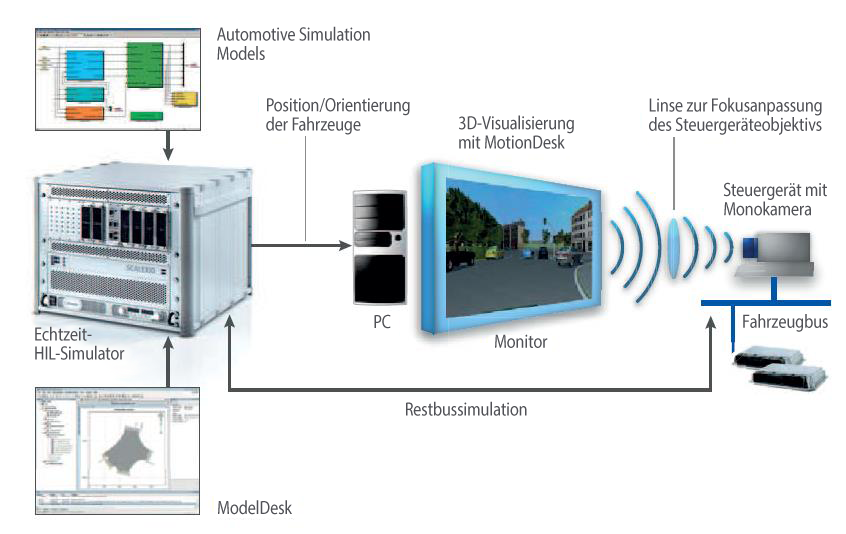
\includegraphics[width=0.8\textwidth]{images/Hil.png}
  %}
  \caption{Schematischer Aufbau eines HIL-Simulators zum Testen von kamera- und radarbasierten Fahrassistenzsystemen~\cite{dSPACEGmbH.2014}}
  \label{fig:HiL}
\end{figure}

Die 3D-Visualisierung wird auf diese Weise zu einem Teil der HIL-Simulation. Die Qualit\"at des Renderings bestimmt somit die Testaussagen \"uber die korrekte Funktionalit\"at des kamerabasierten Systems. Dies trifft insbesondere auf die Qualit\"at des verwendeten Beleuchtungsmodells zu~\cite{Nentwig.2014}.
Des Weiteren kann der Entwicklungszyklus des Fahrerassistenzsystems \"uber eine m\"oglichst realistische Darstellung verk\"urzt werden, da weniger Testfahrten mit realen Fahrzeugen unternommen werden m\"ussen~\cite{dSPACEGmbH.2013}.



\clearpage
\textbf{Betreuung:}

\begin{tabular}{p{14cm}}\\
 \rule{0pt}{18pt}\textit{Erstgutachterin:} 		\\
 \rule{0pt}{14pt}Prof. Dr. Gitta Domik	\\
\rule{0pt}{14pt}Universität Paderborn	\\
Fakultät für Elektrotechnik, Informatik und Mathematik \\
Fürstenallee 11				\\
33102 Paderborn				\\
Tel. 05251-606610				\\
domik@uni-paderborn.de		 	
\end{tabular}\\ [0.1cm]


\begin{tabular}{p{14cm}}\\
 \rule{0pt}{18pt}\textit{Betreuerin:} 		\\
 \rule{0pt}{14pt}Sabrina Heppner, M. Sc.	\\
\rule{0pt}{14pt}Universität Paderborn	\\
Fakultät für Elektrotechnik, Informatik und Mathematik \\
Fürstenallee 11				\\
33102 Paderborn				\\
Tel. 05251-606323				\\
sheppner@mail.uni-paderborn.de	
\end{tabular}\\ [0.8cm]

\begin{tabular}{p{7cm}}
 \rule{0pt}{18pt}\textit{Zweitgutachterin} 		\\
 \rule{0pt}{14pt}Prof. Dr. Ingrid Scharlau	\\
\rule{0pt}{14pt}Universität Paderborn	\\
Warburger Str. 100				\\
33102 Paderborn					\\
Tel. 05251-602900				\\
 ingrid.scharlau@uni-paderborn.de				
\end{tabular}\\[0.4cm]


\clearpage

\section{Literaturverzeichnis}
  \vspace*{-8mm}
\renewcommand{\refname}{}
\renewcommand{\thepage}{}
  \bibliography{literatur}
\bibliographystyle{alphadinSH}


\end{document}